%! Author = amatarazzo
%! Date = 09/05/24

\chapter{Utilization Strategies and Techniques}
\label{ch:utilization}

\section{Introduction}
\label{sec:ch4-introduction}

In this chapter, we will discuss the strategies and techniques that can be used to utilize large language models effectively.
We will start by discussing the importance of context in utilizing large language models and how it can be used to improve their performance.
We will then move on to the concept of chain-of-thought prompting and how it can be used to guide the generation of text.
Finally, we will discuss the importance of planning for complex tasks and how it can be used to improve the performance of large language models.

\section{In-Context Learning}
\label{sec:in-context-learning}
In-context learning is a special prompting technique, initially introduced by \textcite{brown2020language}, that allows the model to learn from the context of the prompt (examples shown in Figure~\ref{fig:in-context-learning}).
\begin{figure}[h!]
	\centering
	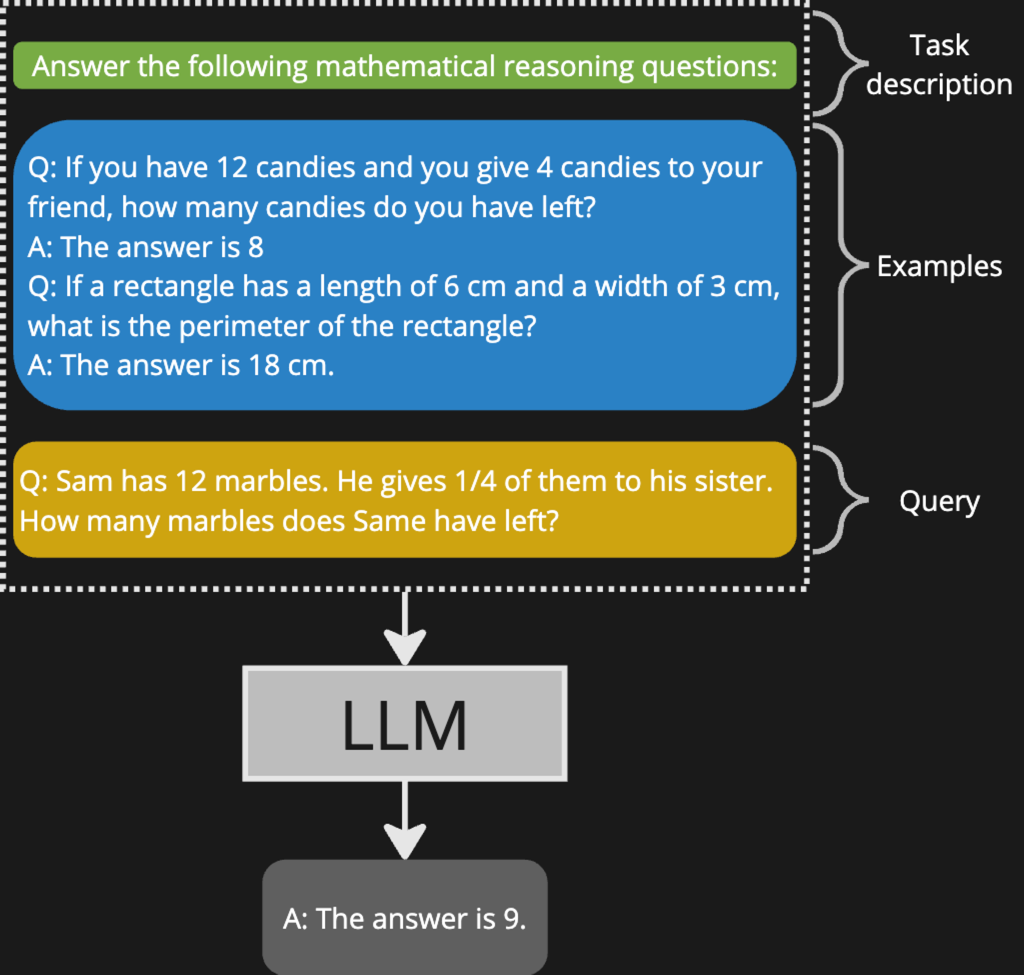
\includegraphics[width=\textwidth]{icl}
	\caption{In-context learning contrasted with traditional fine-tuning. Source: \textcite{brown2020language}}
	\label{fig:in-context-learning}
\end{figure}
As stated in \textcite{brown2020language}, ICT consists of the task description and/or few examples of the task as demonstrations combined in a specific order to form natural language prompts with specifically designed templates.
Finally, the test instance is appended to the prompt to form the input for LLMs to generate the output.

\begin{table}[h!]
	\centering
	\tiny
	\begin{tabularx}{\textwidth}{|l|X|X|}
		\hline
		\textbf{Approach}                         & \textbf{Representative Work}                                                                                                                                                                                                                                                                                                                                                                                                                 & \textbf{Key Point}                                                                                                                                                                                                                                                                                                                                                                                                                                                                                                                                                                                                                                                                                                                                                                                                                                                          \\
		\hline
		\textbf{In-context Learning (ICL)}        & KATE~\cite{liu2022good}, EPR~\cite{rubin2022learning}, SG-ICL~\cite{kim2022self}, APE~\cite{zhou2023large}, Structured Prompting~\cite{hao2022structured}, GlobalE \& LocalE~\cite{lu2022fantastically}                                                                                                                                                                                                                                      & Demonstration selection (similar, k-NN) \newline Demonstration selection (dense retrieval; contrastive learning) \newline Demonstration selection (LLM as the demonstration generator) \newline Demonstration format (automatic generation \& selection) \newline Demonstration format (grouped context encoding; rescaled attention) \newline Demonstration order (entropy-based metric; probing set generation with LLM)                                                                                                                                                                                                                                                                                                                                                                                                                                                  \\
		\hline
		\textbf{Chain-of-thought Prompting (CoT)} & Complex CoT~\cite{fu2022complexity}, Auto-CoT~\cite{zhang2022automatic}, Selection-Inference~\cite{creswell2022selection}, Self-consistency~\cite{wang2022self}, DIVERSE~\cite{li2022advance}, Rationale-augmented ensembles~\cite{wang2022rationale}                                                                                                                                                                                        & Demonstration (complexity-based selection) \newline Demonstration (automatic generation) \newline Generation (alternate between selection and inference) \newline Generation (diverse paths; self-ensemble) \newline Generation (diverse paths; Verification (step-wise voting)) \newline Generation (rationale sampling)                                                                                                                                                                                                                                                                                                                                                                                                                                                                                                                                                   \\
		\hline
		\textbf{Planning}                         & Least-to-most prompting~\cite{zhou2022least}, DECOMP~\cite{khot2022decomposed}, PS~\cite{wang2023plan}, Faithful CoT~\cite{lyu2023faithful}, PAL~\cite{gao2022pal}, HuggingGPT~\cite{shen2023hugginggpt}, AdaPlanner~\cite{sun2023adaplanner}, TIP~\cite{lu2023multimodal}, RAP~\cite{hao2023reasoning}, ChatCoT~\cite{chen2023chatcot}, ReAct~\cite{yao2022react}, Reflexion~\cite{shinn2023reflexion}, Tree of Thoughts~\cite{yao2023tree} & Plan generation (text-based; problem decomposition) \newline Plan generation (text-based; problem decomposition) \newline Plan generation (text-based) \newline Plan generation (code-based) \newline Plan generation (code-based; Python) \newline Plan generation (code-based; models from HuggingFace) \newline Plan refinement (skill memory) \newline Feedback acquisition (visual perception) \newline Feedback acquisition (LLM as the world model; Plan refinement (Monte Carlo Tree Search)) \newline Feedback acquisition (tool); Plan refinement (conversation between LLM and tools) \newline Feedback acquisition (tool); Plan refinement (synergizing reasoning and acting) \newline Feedback acquisition (text-based self-reflection); Plan refinement (dynamic memory) \newline Feedback acquisition (vote comparison); Plan refinement (tree-based search) \\
		\hline
	\end{tabularx}
	\caption{Typical LLM utilization methods and their key points for ICL, CoT, and planning. Note that the key points only highlight the most important technical contribution. Source: \textcite{survey}}
	\label{tab:utilization-methods}
\end{table}

Based on task demonstrations, LLMs can learn to perform a new task without explicit gradient update.
Formally, the in-context learning task can be defined as follows:
\begin{equation}
	LLM(I, \underbrace{f(x_1, y_1), \dots, f(x_k, y_k)}_\text{demonstrations}, \underbrace{f(x_{k+1}}_\text{input}, \underbrace{\uline{~~~}}_\text{answer})) \rightarrow \hat{y}_{k+1}
	\label{eq:ict}
\end{equation}
where $I$ is a task description, $f(x_i, y_i)$ function that convert task demonstration to natural language, $x_{k+1}$ is a new input query, $\hat{y}_{k+1}$ is the prediction of the output generated, and the actual answer $y_{k+1}$ is left as a blank to be predicted by the LLM\@.

\begin{figure}[h!]
	\centering
	\resizebox{\textwidth}{!}{
		\begin{forest}
			forked edges,
			for tree={
					grow=east,
					reversed=true, % reverse the direction of growth
					anchor=base west, % align text to the west
					parent anchor=east,
					child anchor=west,
					base=left,
					font=\small,
					rectangle,
					draw,
					align=left,
					s sep=3mm, % sibling distance
					l sep=10mm, % level distance
					inner xsep=3mm, % text padding horizontal
					inner ysep=1mm  % text padding vertical
				}
				[In-context Learning
						[Inference
								[Scoring Function
										[{Channel prompt tuning~\cite{min2022metaicl},\\
													kNN-Prompting~\cite{xu2023knn}}]
								]
								[Demonstration Designing
										[Organization
												[Selecting
														[{KATE~\cite{liu2022good}, \\
																	EPR~\cite{rubin2022learning}, \\
																	PPL~\cite{gonen2022demystifying}, \\
																	SG-ICL~\cite{kim2022selfgenerated}, \\
																	Self Adaptive~\cite{wu2022selfadaptive}, \\
																	MI~\cite{sorensen2022information}, \\
																	Q-Learning~\cite{zhang2022active}, \\
																	Informative Score~\cite{li2023finding}, \\
																	Topic~\cite{wang2023large}, \\
																	UDR~\cite{li2023finding}}]
												]
												[Ordering
														[{GlobalE\&LocalE~\cite{lu2022fantastically}}]
												]
										]
										[Formatting
												[Instruction
														[{Instruction Induction~\cite{honovich2022instruction}, \\
																	APE~\cite{zhou2022least}, \\
																	Self-Instruct~\cite{wang2022selfinstruct}}]
												]
												[Reasoning Steps
														[{CoT~\cite{wang2022selfinstruct}, \\
																	Complex CoT~\cite{fu2022complexity}, \\
																	AutoCoT~\cite{zhang2022automatic}, \\
																	Self-Ask~\cite{press2022train}, \\
																	MoT~\cite{li2023mot}, \\
																	SuperICL~\cite{xu2023small}, \\
																	iCAP~\cite{wang2022iteratively}, \\
																	Least-to-Most Prompting~\cite{zhou2022least} }]
												]
										]
								]
						]
						[Training
								[Warmup
										[Self-supervised In-context Training
												[{Self-supervised ICL~\cite{chen2022improving}, \\
															PICL~\cite{gu2023pretraining}}]
										]
										[Supervised In-context Training
												[{MetaICL~\cite{min2022metaicl}, \\
															OPT-IML~\cite{iyer2022opt}, \\
															FLAN~\cite{wei2022fine}, \\
															Super-NaturalInstructions~\cite{wang2022super}, \\
															Scaling Instruction~\cite{chung2022scaling}, \\
															Symbol Tuning~\cite{wei2023symbol}}]
										]
								]
						]
				]
		\end{forest}
	}
	\caption{Taxonomy of in-context learning. The training and the inference stage are two main stages for ICL. During the training stage, existing ICL studies mainly take a pretrained LLM as backbone, and optionally warmup the model to strengthen and generalize the ICL ability. Towards the inference stage, the demonstration designing and the scoring function selecting are crucial for the ultimate performance. Source: \textcite{dong2023survey}}
	\label{fig:icl-taxonomy}
\end{figure}

Since the performance of ICL heavily relies on demonstrations, it is important to properly design them in the prompts.
The tree main aspects are a direct consequence of what defined in the the Equation~\ref{eq:ict}: how to select the task demonstrations, how to convert them into natural language, and arrange demonstrations in a reasonable order.

Different training strategies enhance ICL capabilities, improving performance across various tasks without specific task optimization during the pre-training phase (see Figure~\ref{fig:icl-taxonomy} under the Training branch).
Main approaches include Supervised In-context Training, such as MetaICL\footnote{Meta-training for InContext Learning} and Symbol Tuning, and Self-supervised In-context Training, such as Self-supervised ICL and PICL~\cite{dong2023survey}.

MetaICL~\cite{min2022metaicl} proposed to continually train LLMs on a wide range of tasks\footnote{Classification, question answering,
	natural language inference, paraphrase detection and more} with demonstration examples.
This approach is related to other works that uses multi-task learning for better zero-shot performance at test time~\cite{min2022metaicl}.
However, MetaICL is distinct as it allows learning new tasks from k examples alone, without relying on a task reformatting (e.g., reducing everything to question answering)
or task-specific templates (e.g., converting different tasks to a language modeling problem).
MetaICL is based on the core idea of in-context learning by conditioning on training examples i.e., explicitly training on an in-context learning objective).

Symbol Tuning~\cite{wei2023symbol} instead fine-tunes language models on in-context input-label pairs, substituting natural language labels (e.g., "positive/negative sentiment") with arbitrary symbols (e.g., "foo/bar").
As a result, symbol tuning demonstrates an enhanced capacity to utilize in-context information for overriding prior semantic knowledge.
Compared to MetaICL, which constructs several demonstration examples for each task, instruction tuning mainly considers an explanation of the task and is more easier to scale up.

Self-supervised ICL leverages raw corpora to generate input/output pairs as training data, while PICL also utilizes raw corpora but employs a simple language modeling objective, promoting task inference and execution based on context.
PICL shown to be more effective in zero-shot settings and tasks generalization~\cite{dong2023survey}.

Effective demonstration design is crucial, involving selecting and ordering examples, or using instruction induction and reasoning steps (as shown in Figure~\ref{fig:icl-taxonomy} under the Inference/ Demonstration Designing branch).
The selection aims to choose good examples for ICL using unsupervised\footnote{Based on pre-defined metrics} or supervised methods.
For example, KATE~\cite{liu2022good} and EPR~\cite{rubin2022learning} select demonstrations based on similarity.
The ordering of the selected demonstrations is also an important aspect of demonstration design.
\textcite{lu2022fantastically} have proven that order sensitivity is a common problem and affects various models.
To handle this problem, studies have proposed several training-free methods to order demonstrations.
\textcite{liu2022good} sorted examples based on similarity, while GlobalE\&LocalE~\cite{lu2022fantastically} orders demonstrations based on global and local entropy.

ICL has a close connection with instruction tuning (discussed in Section~\ref{subsec:instruction-tuning}) in that both utilize natural language to format the task or instances.
However, instruction tuning needs to fine-tune LLMs for adaptation, while ICL only prompts LLMs for utilization~\cite{survey}.
Furthermore, instruction tuning can enhance the ICL ability of LLMs to perform target tasks, especially in the zero-shot setting\footnote{Using only task descriptions}~\cite{chung2022scaling}.

\section{Chain-of-Thought prompting}
\label{sec:chain-of-thought}
\lipsum

\section{Planning for complex tasks}
\label{sec:planning}
\lipsum